
%(BEGIN_QUESTION)
% Copyright 2012, Tony R. Kuphaldt, released under the Creative Commons Attribution License (v 1.0)
% This means you may do almost anything with this work of mine, so long as you give me proper credit

Determine the amount of work done stretching a spring from 3 inches of stretch to 5 inches of stretch, given the plot of force versus stretch shown here.  This spring happens to have a constant $k$ of 1 pounds per inch (1 additional pound of force required to stretch it each additional inch):

$$\includegraphics[width=15.5cm]{i01888x01.eps}$$

Choose the closest answer:

\begin{itemize}
\item{} -2 inch-pounds
\vskip 10pt 
\item{} +12.5 inch-pounds
\vskip 10pt 
\item{} +8 inch-pounds
\vskip 10pt 
\item{} +4.5 inch-pounds
\vskip 10pt 
\item{} +6 inch-pounds
\vskip 10pt 
\item{} +2 inch-pounds
\vskip 10pt 
\item{} -4.5 inch-pounds
\end{itemize}

\underbar{file i01888}
%(END_QUESTION)





%(BEGIN_ANSWER)

+8 inch-pounds

%(END_ANSWER)




%(BEGIN_NOTES)

{\bf This question is intended for exams only and not worksheets!}.

%(END_NOTES)


